\documentclass{bmcart}

%%%%%%%%%%%%%%%%%%%%%%%%%%%%%%%%%%%%%%%%%%%%%%
%%                                          %%
%% CARGA DE PAQUETES DE LATEX               %%
%%                                          %%
%%%%%%%%%%%%%%%%%%%%%%%%%%%%%%%%%%%%%%%%%%%%%%

%%% Load packages
\usepackage{amsthm,amsmath}
\usepackage{graphicx}
%\RequirePackage[numbers]{natbib}
%\RequirePackage{hyperref}
\usepackage[utf8]{inputenc} %unicode support
%\usepackage[applemac]{inputenc} %applemac support if unicode package fails
%\usepackage[latin1]{inputenc} %UNIX support if unicode package fails


%%%%%%%%%%%%%%%%%%%%%%%%%%%%%%%%%%%%%%%%%%%%%%
%%                                          %%
%% COMIENZO DEL DOCUMENTO                   %%
%%                                          %%
%%%%%%%%%%%%%%%%%%%%%%%%%%%%%%%%%%%%%%%%%%%%%%

\begin{document}

	\begin{frontmatter}
	
		\begin{fmbox}
			\dochead{Research}
			
			%%%%%%%%%%%%%%%%%%%%%%%%%%%%%%%%%%%%%%%%%%%%%%
			%% INTRODUCIR TITULO PROYECTO               %%
			%%%%%%%%%%%%%%%%%%%%%%%%%%%%%%%%%%%%%%%%%%%%%%
			
			\title{Implicación del gen que codifica la subunidad beta-3 de la proteína G (GNB3) en los mecanismos de la diabetes materna}
			
			%%%%%%%%%%%%%%%%%%%%%%%%%%%%%%%%%%%%%%%%%%%%%%
			%% AUTORES. METER UNA ENTRADA AUTHOR        %%
			%% POR PERSONA                              %%
			%%%%%%%%%%%%%%%%%%%%%%%%%%%%%%%%%%%%%%%%%%%%%%
			
			\author[
			  addressref={aff1},                   % ESTA LINEA SE COPIA IGUAL PARA CADA AUTOR
			  corref={aff1},                       % ESTA LINEA SOLO DEBE TENERLA EL COORDINADOR DEL GRUPO
			  email={victorgo@uma.es}   % VUESTRO CORREO ACTIVO
			]{\inits{V.G.O}\fnm{Víctor} \snm{Guirado Osorio}} % inits: INICIALES DE AUTOR, fnm: NOMBRE DE AUTOR, snm: APELLIDOS DE AUTOR
			\author[
			  addressref={aff2},
			  email={susanafernandez@uma.es}
			]{\inits{S.R.F.G}\fnm{Susana R.} \snm{Fernández Giaccomassi}}
			\author[
			addressref={aff3},
			email={pablobermudezgamez@uma.es}
			]{\inits{P.B.G}\fnm{Pablo} \snm{Bermúdez Gámez}}
			\author[
			addressref={aff4},
			email={juancavergara6@uma.es}
			]{\inits{J.C.V.R}\fnm{Juan C.} \snm{Vergara Ruz}}
			
			%%%%%%%%%%%%%%%%%%%%%%%%%%%%%%%%%%%%%%%%%%%%%%
			%% AFILIACION. NO TOCAR                     %%
			%%%%%%%%%%%%%%%%%%%%%%%%%%%%%%%%%%%%%%%%%%%%%%
			
			\address[id=aff1]{%                           % unique id
			  \orgdiv{ETSI Informática},             % department, if any
			  \orgname{Universidad de Málaga},          % university, etc
			  \city{Málaga},                              % city
			  \cny{España}                                    % country
			}
		
		\end{fmbox}% comment this for two column layout
		
		\begin{abstractbox}
		
			\begin{abstract} % abstract
			
			
			Durante el embarazo, diversos mecanismos fisiológicos se ven afectados, incluyendo la regulación de leptina, adiponectina y la gluconeogénesis, lo que puede desencadenar complicaciones relacionadas con la diabetes materna (DM). Un mecanismo biológico de particular interés es la posible relación entre la DM y el gen GNB3, que está implicado en la ganancia de peso y la obesidad, factores que son conocidos por incrementar la resistencia a la insulina. Esto sugiere la necesidad de una mayor investigación para comprender mejor la contribución del gen GNB3, profundizando en su papel en la regulación de la glucosa y su influencia en el desarrollo de la DM.
			
			
			\end{abstract}
			
			%%%%%%%%%%%%%%%%%%%%%%%%%%%%%%%%%%%%%%%%%%%%%%
			%% PALABRAS CLAVE DEL PROYECTO              %%
			%%%%%%%%%%%%%%%%%%%%%%%%%%%%%%%%%%%%%%%%%%%%%%
			
			\begin{keyword}
			\kwd{diabetes materna}
			\kwd{insulina}
			\kwd{GNB3}
			\end{keyword}
		
		
		\end{abstractbox}
	
	\end{frontmatter}
	
	
	%%%%%%%%%%%%%%%%%%%%%%%%%%%%%%%%%
	%% COMIENZO DEL DOCUMENTO REAL %%
	%%%%%%%%%%%%%%%%%%%%%%%%%%%%%%%%%
	
	\section{Introducción}

La diabetes materna (DM) o diabetes gestacional (HP:0009800), es un trastorno que afecta a la secreción y la función de la insulina, conduciendo a la hiperglucemia \cite{Rodolaki2023}. Se caracteriza por su aparición en mujeres previamente normoglucémicas \cite{Rodolaki2023}, tratándose de cualquier grado de intolerancia a la glucosa que se desarrolle por primera vez durante el embarazo \cite{ADB2009}, y que no sea claramente diabetes manifiesta \cite{Grazia2020}. Durante el embarazo se ve un aumento de hormonas locales y placentarias que conlleva a un estado de resistencia a la insulina, elevando los niveles de glucosa en sangre para soportar las demandas del feto \cite{Plows2018}. Después de un embarazo saludable, la sensibilidad a la insulina vuelve a los niveles previos, mientras que en algunos casos no ocurre así, resultando en DM \cite{Plows2018}.


Se estima que el gasto en salud en personas diabéticas a nivel mundial en 2017 fue de 850 mil millones de dólares \cite{Cho2018} y que las mujeres que padecen diabetes durante la gestación tienen diez veces más riesgo de desarrollar diabetes mellitus tipo 2 (DMT2) que mujeres con un embarazo normal \cite{Vounzoulaki2020} \cite{You2021}. La prevalencia de hiperglucemia en el embarazo entre mujeres de 20 a 49 años es de un 16% y la cifra va en aumento \cite{Guariguata2014}.

Se asocia a la DM con enfermedades cardiacas en el feto \cite{Depla2021} e incluso con enfermedades cardiovasculares y cerebrovasculares en la madre \cite{Xie2022}.

	\section{Materiales y métodos}

\subsection{Materiales}
Se utilizaron datos biológicos relacionados con el fenotipo "Maternal diabetes" (HP:0009800), los cuales fueron extraídos de la base de datos Human Phenotype Ontology (HPO) en la web hpo.jax\cite{Kohler2017}. Específicamente, se trabajó con una lista de 43 genes asociados al fenotipo, la cual se encontraba en formato Excel. Asimismo, se incorporó el identificador de nuestro gen (GNB3) en este contexto.

Para el análisis bioinformático, se utilizaron diversas herramientas y software, entre los que destacan:

\begin{itemize}
	\item La API de StringDB\cite{Szklarczyk2015} como la herramienta principal.
	\item Python, con las librerías openpyxl 3.1.2, Stringdb 0.1.5\cite{Mering2005}, Pandas 2.1.2\cite{McKinney2015}, iGraph 0.11.2\cite{Csardi2006}, Cairocffi 1.6.1, para el procesamiento de datos y las representaciones.
	\item El algoritmo de detección de comunidades "community edge betweenness"~\cite{Girvan2002} implementado en iGraph.
\end{itemize}

La configuración e instalación necesarias se llevaron a cabo mediante scripts en Bash\cite{Dong2023}.

Los análisis se llevaron a cabo en un entorno computacional que consistía en sistemas con [HARDWARE] y utilizando el sistema operativo Ubuntu 23.

\subsection{Metodología}

EL flujo de trabajo que se siguió puede observarse en la figura \ref{fig:workflow} y que se explicará en detalle a continuación.

\begin{figure}[h!]
	\includegraphics[width=0.9\textwidth]{figures/workflow.png}
	\caption{Flujo de trabajo: Se representa el flujo de trabajo seguido para la realización del proyecto. Empieza desde la obtención de los genes asociados al fenotipo de interés y la creación de la red de interacción hasta el análisis por enriquecimiento funcional.}
	\label{fig:workflow}
\end{figure}

Descargamos la lista de genes implicados al fenotipo HP:0009800 directamente desde HPO en formato excel.

Utilizamos la librería de Python de stringdb mediante el método "get\_network" para realizar una petición a su API para obtener la red de interacción de los genes asociados al fenotipo a la que previamente se insertó el gen GNB3 para realizar su estudio.

Mediante la librería de igraph se construyó la red de interacción de genes y se realizó un algoritmo de detección de comunidades basado en "edge betweenness". Una vez realizado la detección, se seleccionó la comunidad donde estaba presente el gen GNB3.

Realzamos un enriquecimiento funcional de los genes que formaban parte de esa comunidad mediante la librería de stringdb mediante el método "get\_enrichment". 

Se creó una nueva red mediante una propagación en red de los genes presente en la comunidad de interés a través del método "get\_network" con un nuevo parámetro de entrada "add\_nodes = 16" para indicar que se añadieron 16 genes más. A partir de esta red volvimos a realizar un enriquecimiento funcional.

	
\section{Resultados}

\subsection{Visión General}

Hemos investigado el uso de la biología de sistemas para entender mejor el fenotipo diabetes materna. En esta sección presentaremos los resultados del análisis de la red de genes relacionados con el fenotipo a partir de datos de interacción proteína-proteína descargados de STRINGdb con el propósito de estudiar la relación entre la diabetes materna y el gen GNB3.

A continuación procederemos a detallar los resultados obtenidos al ejecutar nuestro flujo de trabajo.

\subsection{Red de interacción}

Al descargar la lista de genes implicados en el fenotipo de estudio, observamos que la cantidad de enfermedades asociadas son 31 y los genes son 43. Hemos generado la red de interacción entre estos genes para obtener la cantidad de nodos e interacciones entre ellos. En la Tabla~\ref{table:nodes_edges_count} se puede observar la cantidad de nodos (genes) y edges (interacciones) de la red sin incluir el gen GNB3 e incluyendo al gen para hacer la red.


\begin{table}[h]
	\centering
	\caption{Cantidad de nodos e interacciones: Se ha creado la red de interacciones de los genes relacionados con el fenotipo y otra red añadiendo al gen de estudio. Finalmente, se ha obtenido la cantidad de nodos y edges de cada red.}
	\label{table:nodes_edges_count}
	\begin{tabular}{|c|c|c|}
		\hline
		\textbf{Red} & \textbf{Nodos} & \textbf{Edges} \\ \hline
		Sin GNB3 & 43    & 272   \\ \hline
		Con GNB3 & 44    & 276  \\ \hline
	\end{tabular}

\end{table}

La red generada por stringdb usando los genes asociados a la diabetes materna y el GNB3 se pude observar en la Figura~\ref{fig:network}.

\begin{figure}[h!]
	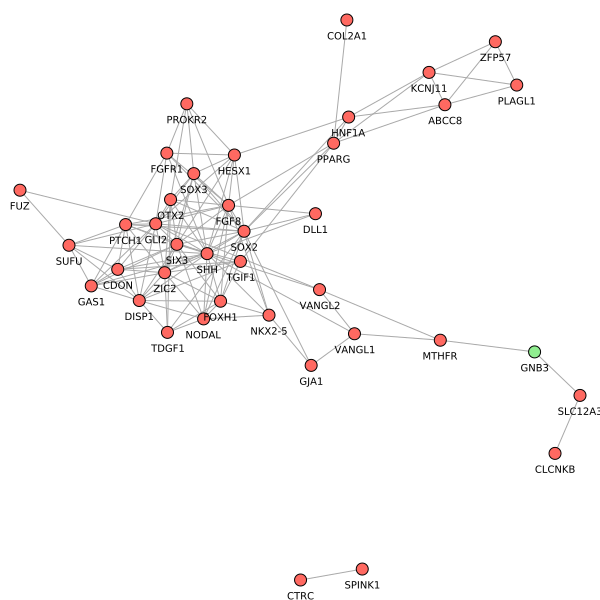
\includegraphics[width=0.9\textwidth]{figures/network.pdf}
	\caption{Red de Interacción: Se observan las interacciones entre los genes asociados al fenotipo de estudio y el gen GNB3. Los nodos en rojo representan los genes asociados al fenotipo, mientras que el nodo verde representa al GNB3.}
	\label{fig:network}
\end{figure}

\subsection{Detección de comunidades}

Hemos detectado las comunidades de la red obtenida en el paso anterior, usando el método ``edge betweenness'' descrito en la sección de métodos. Obtuvimos cinco comunidades a partir de la red de interacciones. El GNB3 se encuentra presente en una comunidad con otros dos nodos, los genes SLC12A3 y el CLCNKB, como puede observarse en la Figura~\ref{fig:comunidad}.

\begin{figure}[h!]
	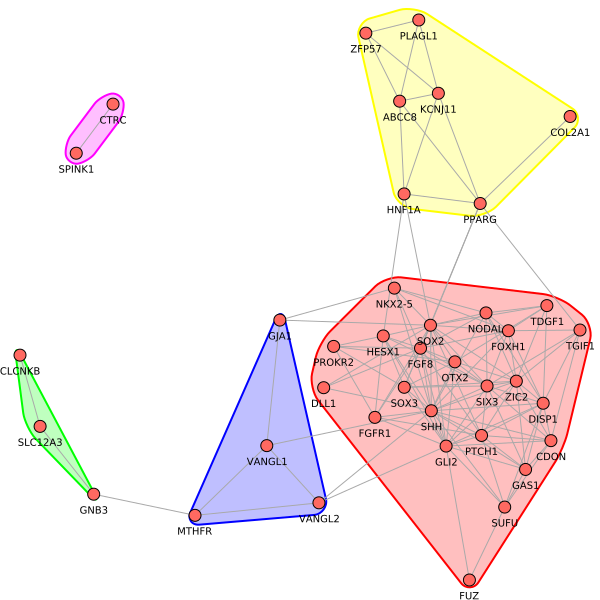
\includegraphics[width=0.9\textwidth]{figures/comunidades.pdf}
	\caption{Detección de comunidades: Se representa la clusterización de los nodos en cinco comunidades.}
	\label{fig:comunidad}
\end{figure}

\subsection{Enriquecimiento funcional}

Una vez detectada la comunidad a la que pertenece el GNB3 en la red de estudio, hemos obtenido el enriquecimiento funcional para los tres genes pertenecientes a la comunidad.  Filtrando aquellos resultados en los que aparece el gen GNB3, el análisis demostró un enriquecimiento para el fenotipo HPO de anormalidad de la visión, con un p-valor de 0.00021, como se puede observar en la Tabla~\ref{table:enriquecimiento1}

\begin{table}[h]
	\centering
	\caption{Enriquecimiento funcional de la comunidad del gen GB3: Se observa el único resultado para el gen de interés.}
	\label{table:enriquecimiento1}
	\begin{tabular}{|c|c|c|c|c|c|}
		\hline
		\textbf{Preferred Names} & \textbf{Description} & \textbf{P-value} & \textbf{fdr} & \textbf{Category} & \textbf{Term} \\ \hline
		GNB3, CLCNKB, SLC12A3 & Abnormality of vision    & 0.00021 & 0.0197&  HPO & HP:0000504 \\ \hline

	\end{tabular}

\end{table}

\subsection{Propagación de la red}

Hemos realizado la propagación de la red añadiendo 16 nodos más, que interaccionan con los tres genes pertenecientes a la comunidad del gen GNB3. A continuación, hemos procedido a realizar el enriquecimiento funcional incluyendo los nuevos genes. En este caso, el gen de interés apareció implicado en 96 procesos, de los cuales se muestran aquellos relacionados con la regulación de insulina y glucagón en la Tabla~\ref{table:enriquecimiento2}. Se puede observar que, en todos los casos representados, hay un enriquecimiento significativo en términos relacionados con RCTM, que ha sido introducido en la sección de métodos.


\begin{table}[h]
	\centering
	\caption{Enriquecimiento funcional de la comunidad del gen GB3 expandida: Se observan los resultados que incluyen al gen GNB3 y que incluyen mecanismos relacionados con la insulina o el glucagón. Todos los resultados son de la categoría RCTM.}
	\label{table:enriquecimiento2}
	\begin{tabular}{|c|c|c|c|}
		\hline
		 \textbf{Description} & \textbf{P-value} &\textbf{ fdr }&  \textbf{Term} \\ \hline
		 Regulation of insulin secretion   & 9.38e-30 & 1.05e-27 &   HSA-422356 \\ \hline
		 Glucagon-like Peptide-1 (GLP1) regulates insulin secretion  & 3.57e-30 & 5.44e-28  & HSA-381676 \\ \hline
		 Adrenaline,noradrenaline inhibits insulin secretion & 3.88e-29 & 3.28e-27  & HSA-400042 \\ \hline
		 Glucagon-type ligand receptors & 2.51e-31 & 5.73e-29  & HSA-420092 \\ \hline
		 Glucagon-like Peptide-1 (GLP1) regulates insulin secretion & 3.57e-30 & 5.44e-28  & HSA-381676 \\ \hline
		 Glucagon signaling in metabolic regulation & 1.31e-25 & 6.95e-24  & HSA-163359 \\ \hline
		 Synthesis, secretion, and inactivation of Glucagon-like Peptide-1 (GLP-1) & 1.33e-06 & 4.39e-05  & HSA-381771 \\ \hline
	\end{tabular}

\end{table}

Después de haber presentado los resultados, la discusión de los mismos seguirá en la próxima sección.

	\section{Discusión}

Hemos encontrado una interacción significativa entre los genes asociados a la DM y el gen GNB3, particularmente en los procesos de regulación de insulina y glucagón. Esta interacción es relevante, ya que estas vías metabólicas están vinculadas con la obesidad, un factor de riesgo conocido para la DM \cite{Shah2011}. Además, los resultados del primer enriquecimiento funcional muestran una asociación entre la DM y complicaciones en la visión, que es un aspecto frecuente en pacientes con DM \cite{Bailes2002}.


El enriquecimiento funcional nos ha proporcionado resultados confiables, ya que todos los procesos obtenidos presentan p-valores y FDR significativos. Al simplificar la red para incluir solo relaciones entre nodos únicos, aumentamos la eficiencia en la detección de comunidades. Este enfoque nos permite centrarnos más en la presencia de relaciones significativas en lugar del número de interacciones.

Una limitación que presenta el estudio es que como no se obtuvieron procesos relacionados con la insulina en el primer enriquecimiento funcional, se realizó una propagación de la comunidad. Esto es un procedimiento correcto, ya que busca más nodos relacionados con la comunidad de estudio para encontrar más información. Sin embargo, este paso fue en parte premeditado; es decir, la ejecución de la propagación sólo se consideró tras obtener y analizar los resultados iniciales.

En vista de nuestros resultados, se abren diversas oportunidades para estudios confirmatorios que consoliden y expandan nuestras observaciones. En primer lugar, recomendamos la validación experimental de las interacciones identificadas entre los genes asociados a la diabetes materna y el gen GNB3 en los mecanismos de regulación de insulina y glucagón. La confirmación de estas interacciones mediante análisis de expresión diferencial \cite{Haynes2013} podría proporcionar una base sólida para futuros estudios clínicos.

Además, es importante abordar las preguntas que aún persisten en nuestra investigación. La propagación de la comunidad, aunque justificada, plantea la pregunta sobre la extensión de la red y la identificación de nuevos nodos relacionados con la diabetes materna. Se requieren estudios adicionales para comprender completamente la complejidad de estas interacciones y su contribución a los fenotipos asociados.

En general, la identificación de mecanismos de regulación de insulina y glucagón relacionados con la DM y la obesidad  \cite{Shah2011} mediante el gen GNB3 sugiere posibles objetivos terapéuticos. Esto no solo podría beneficiar a las personas con DM, sino también a aquellos en riesgo de desarrollar obesidad relacionada con problemas metabólicos. Los resultados de nuestro estudio pueden orientar estrategias preventivas y terapéuticas, mejorando la calidad de vida de las personas afectadas.


	\section{Conclusiones}

En conclusión, aceptamos nuestra hipótesis inicial pues nuestros hallazgos respaldan la asociación entre los genes relacionados con la diabetes materna y el gen GNB3 mediante los procesos de regulación metabólica de la insulina y el glucagón. La fuerza estadística de nuestros resultados obtenidos por análisis de enriquecimiento funcional significativos, complementa la validez de nuestras observaciones. Esta investigación sienta las bases para futuras exploraciones tanto a nivel experimental como clínico.

Reiteramos la importancia de considerar los resultados en el contexto de posibles aplicaciones terapéuticas y destacamos la relevancia de la gestión de la diabetes materna para abordar problemas metabólicos durante el embarazo. En última instancia, destacar que nuestros hallazgos sobre las redes de interacciones genéticas subyacentes a la diabetes materna, proporcionan conocimientos clave para la comprensión de la enfermedad y sus implicaciones en la salud.


	
	
	%%%%%%%%%%%%%%%%%%%%%%%%%%%%%%%%%%%%%%%%%%%%%%
	%% OTRA INFORMACIÓN                         %%
	%%%%%%%%%%%%%%%%%%%%%%%%%%%%%%%%%%%%%%%%%%%%%%
	
	\begin{backmatter}
	
		\section*{Abreviaciones}%% if any
		DM: diabetes materna
		DMT2: diabetes mellitus tipo 2
		
		\section*{Disponibilidad de datos y materiales}%% if any
			%https://github.com/ElArquitectorgo/systems_biology.git
		
		\section*{Contribución de los autores}
			V.G.O : introducción; S.R.F.G : introducción; P.B.G : introducción; J.C.V.R : introducción
		
		
		%%%%%%%%%%%%%%%%%%%%%%%%%%%%%%%%%%%%%%%%%%%%%%%%%%%%%%%%%%%%%%%%%%%%%%%%%%%%%%%%%%%%%%%%
		%% BIBLIOGRAFIA: no teneis que tocar nada, solo sustituir el archivo bibliography.bib %%
		%% por el que hayais generado vosotros                                                %%
		%%%%%%%%%%%%%%%%%%%%%%%%%%%%%%%%%%%%%%%%%%%%%%%%%%%%%%%%%%%%%%%%%%%%%%%%%%%%%%%%%%%%%%%%
		
		\bibliographystyle{bmc-mathphys} % Style BST file (bmc-mathphys, vancouver, spbasic).
		\bibliography{bibliography}      % Bibliography file (usually '*.bib' )
	
	\end{backmatter}
\end{document}
